\documentclass[10pt,a4paper]{article}
\usepackage[margin=1.95cm,top=2.2cm,bottom=2.05cm]{geometry}
\usepackage[T1]{fontenc}
\usepackage{lmodern,microtype,booktabs,tabularx,array,graphicx,xcolor}
\usepackage{enumitem,caption,fancyhdr,xurl,float,amsmath,needspace}
\usepackage[unicode,colorlinks=true,urlcolor=blue!65!black,linkcolor=black]{hyperref}
\graphicspath{{../analysis/figures/}}
\definecolor{ink}{HTML}{202A32}
\definecolor{navy}{HTML}{173E56}
\definecolor{muted}{HTML}{586974}
\definecolor{rule}{HTML}{CED8DD}
\color{ink}
\setlength{\parindent}{0pt}
\setlength{\parskip}{0.24em}
\setlength{\emergencystretch}{2em}
\renewcommand{\arraystretch}{1.14}
\captionsetup{font=small,labelfont=bf}
\setlist[itemize]{leftmargin=1.25em,itemsep=0.1em,topsep=0.15em}
\pagestyle{fancy}
\setlength{\headheight}{22pt}
\fancyhf{}
\fancyhead[L]{\footnotesize\color{muted} IIB423T-1 \quad / \quad C1}
\fancyhead[R]{\footnotesize\color{muted} Medina \& Castillo}
\fancyfoot[R]{\footnotesize\color{muted}\thepage}
\renewcommand{\headrulewidth}{0.35pt}
\renewcommand{\headrule}{\hbox to\headwidth{\color{rule}\leaders\hrule height \headrulewidth\hfill}}
\newcommand{\sectionhead}[1]{\Needspace{8\baselineskip}\vspace{0.33em}{\large\bfseries\color{navy}#1}\par\vspace{0.08em}}
\newcommand{\subhead}[1]{\vspace{0.15em}{\bfseries #1}\par}
\newcommand{\source}[1]{\textsuperscript{[#1]}}

\begin{document}
\thispagestyle{empty}
{\small\bfseries\color{navy} BUSINESS INTELLIGENCE \hspace{0.7em} / \hspace{0.7em} C1 ANALYTICAL REPORT}\par
\vspace{0.6em}
{\LARGE\bfseries Customer concentration in recorded purchase value}\par
\vspace{0.3em}
{\large A reproducible preparation and diagnostic EDA of UCI Online Retail}\par
\vspace{0.55em}
{\color{muted} Mois\'{e}s Medina \quad and \quad Ignacia Castillo \hfill 27 September 2026}\par
\vspace{0.55em}{\color{rule}\hrule height 0.65pt}\vspace{0.55em}

\textbf{Decision in brief.} In the observed 12-month case, the highest-value 10\% of identifiable customers (430 of 4,293 IDs) account for \textbf{60.5\%} of eligible known-ID purchase value. This is a useful signal for a retrospective account review, conditional on the fact that IDs cover only \textbf{85.7\%} of eligible value. We do not interpret the indicator as profit, loyalty, churn, lifetime value or a causal effect of account management. Our source, rules, diagnostics and alternative populations are recorded in the accompanying code and executed notebook.

\sectionhead{1\quad From W1 to C1: why this question}
In W1 we selected UCI Online Retail for its traceable download, dictionary, citation and licence.\source{1} Initial checks of invoice lines, dates, IDs, prices and C flags led to two decisions using the same file: review \emph{customer-value concentration} (A) or monitor \emph{where C-coded cancellation records appear} (B). Their populations and decisions differ.

\begin{table}[H]\centering\small
\caption{W1 choice carried into C1. Both candidates remained descriptive.}
\begin{tabularx}{\linewidth}{@{}p{1.75cm}XX@{}}\toprule
 & A: customer portfolio & B: cancellation records \\\midrule
Decision & Which accounts warrant a closer portfolio review? & Which months or countries warrant a process review? \\
Evidence & Positive priced lines can be ranked by ID and counted by invoice. & C-coded records can be counted by invoice and date. \\
Limit & Missing IDs bound the customer population. & No original-purchase link or cancellation reason; no matched rate. \\
\bottomrule\end{tabularx}
\end{table}

We advanced A because its denominator and missing-ID boundary can be measured and stress-tested. B remains a valid descriptive operations question, but C counts cannot establish a purchase-level cancellation rate or financial loss. We also set aside a November/Christmas explanation: one cycle cannot establish seasonality, and the final December ends after nine days. Monthly values remain context. C1 now tests A's population, KPI and EDA.

\subhead{Documentary basis and policy boundary}
Chen, Sain and Guo's 2012 retail study uses recency, frequency and monetary information to motivate customer segmentation from transaction records.\source{3} It supports investigating a customer portfolio, but it does not validate our particular extract, merchandise rule or KPI. Research on supplier firms also finds that customer concentration can bring both relationship benefits and exposure to major customers.\source{4} Its manufacturing setting differs from this anonymous gift retailer; we therefore use it to motivate a question, not to label 60.5\% safe or dangerous. This is a UK retail case, with no direct relationship to a Chilean MINSAL health priority. We do not attribute a MINSAL objective or numerical target to it. No case-specific instructor response to our W1 selection was documented by 27 September 2026; we retain A provisionally and leave the retail-domain fit and KPI use for instructor discussion.

\sectionhead{2\quad Business framing: from strategy to an indicator}
UCI describes a UK-based non-store gift retailer with many wholesale customers, but does not publish this firm's mission, vision, management targets or account strategy.\source{1} We therefore use a \emph{proposed decision scenario}, not a claim about the firm's actual plan: a commercial team wants to know whether recorded purchase value relies heavily on a small group of identifiable accounts. That matters because losing or changing a major account could affect the observed portfolio, although this file cannot quantify future risk.

\begin{table}[H]\centering\small
\caption{Decision chain proposed for this case; no corporate target is attributed to the retailer.}
\begin{tabularx}{\linewidth}{@{}>{\raggedright\arraybackslash}p{2.45cm}X@{}}\toprule
Element & Operational meaning \\\midrule
Strategic priority & Understand dependence on major accounts before considering portfolio actions. \\
Objective & Measure concentration of recorded positive priced merchandise value among identifiable customers. \\
Question & What share of known-ID value is contributed by the highest-value 10\% of observed IDs? \\
Provisional KPI & Top-decile known-ID value share over a specified observation window. \\
Validity guardrail & Share of all eligible purchase value linked to a customer ID. \\
Decision & Inspect the largest accounts and data coverage when concentration changes; do not automate a customer intervention from this statistic. \\
\bottomrule\end{tabularx}
\end{table}

\Needspace{11\baselineskip}Let $E$ be the eligible positive priced purchase lines, $E_i$ those with customer ID $i$, and $v_j=q_jp_j$ for quantity $q_j$ and sterling unit price $p_j$. Rank the $N$ identifiable customers by $V_i=\sum_{j\in E_i}v_j$. Our indicator and coverage check are
\[
K_{10}=\frac{\sum_{i\in\mathrm{top}\,\lceil 0.10N\rceil}V_i}{\sum_{i=1}^{N}V_i},
\qquad
C_{ID}=\frac{\sum_{j\in E:\,ID_j\,\mathrm{known}}v_j}{\sum_{j\in E}v_j}.
\]
The top-decile convention is an interpretable portfolio benchmark, not a naturally occurring customer class. We round up to whole IDs so that at least 10\% are included. The numerator and denominator use the \emph{same} eligible, known-ID population; otherwise a missing ID would silently change the indicator. We report $C_{ID}$ alongside $K_{10}$ because a high concentration among known IDs might coexist with systematically different unknown-ID purchases.

\subhead{Review rule and target status}
At a future monthly refresh, we would recompute $K_{10}$ on a trailing 12-month window and report $C_{ID}$ and $N$ beside it. Any rise relative to the preceding comparable window would trigger a \emph{diagnostic review} of the accounts contributing most, product-code eligibility and ID coverage. A fall in coverage would trigger a data-capture review before a business interpretation. We set no performance target or automatic spending rule: one historical window supplies neither a management objective nor an intervention-cost model. This is a provisional KPI because it has a proposed objective, cadence and review action; its operational thresholds remain to be agreed with a decision-maker.

\subhead{Seven-step map from Class 03}
The steps below make the chain from a proposed decision to an observed measure explicit.\source{2}\source{5}
\begin{table}[H]\centering\small
\caption{Seven steps applied to this case; the decision is a proposal, not the retailer's published practice.}
\begin{tabularx}{\linewidth}{@{}p{2.65cm}X@{}}\toprule
Step & Case application and boundary \\\midrule
1. Decision & A proposed commercial analyst would review major accounts, first checking whether an apparent concentration change reflects account values or missing IDs. Alternatives are an account review, a data-capture review, or no action pending better evidence. \\
2. Success criteria & Better visibility of dependence and stable ID capture would help the proposed decision. $K_{10}$ and $C_{ID}$ describe the present record; neither demonstrates improved profitability or an achieved business target. \\
3. Business questions & Main: what share of known-ID positive purchase value comes from the highest-value 10\% of observed IDs? Support: how skewed are customer totals, how does invoice frequency relate to value, and how complete are IDs by month? \\
4. Business process & The source records items or adjustments on invoices. We observe line creation, invoice number and date; we do not observe payment settlement, delivery, cost, a linked original purchase for each C record, or account interventions. \\
5. Entities, events and states & An item code appears on an invoice line; lines group into invoices and known IDs group invoices into observed customer records. We flag positive purchase, C-coded negative and other lines. An ID is a recorded key, not verified evidence of a unique person. \\
6. Data representation & One source row is one invoice line with eight original fields. \texttt{InvoiceNo} groups lines; \texttt{CustomerID} groups identifiable purchases. We aggregate within this source after checking the invoice-to-ID mapping; no external join is needed. \\
7. Measurement & On Dec 2010--Nov 2011 eligible lines, $K_{10}$ divides top-$\lceil0.10N\rceil$ known-ID value by all known-ID value; $C_{ID}$ divides known-ID eligible value by all eligible value. Values are in pounds; shares are percentages. Exclusions and interpretations are detailed below. \\
\bottomrule\end{tabularx}
\end{table}

\sectionhead{3\quad Source, population and data-generating process}
We use Daqing Chen's \emph{Online Retail} dataset from UCI, licensed CC BY 4.0. UCI describes 541,909 transaction records from 1 December 2010 to 9 December 2011 and defines an invoice number beginning with C as a cancellation.\source{1} Our supplied extract retains every source row from \textbf{1 December 2010 through 30 November 2011}: 516,384 rows and all eight original columns. We omit only the final nine-day December 2011 fragment so monthly descriptions compare complete calendar months. Month lengths still differ, and a single cycle cannot establish annual seasonality. The extract and its SHA-256 are in \texttt{data/}; the script checks its schema and date bounds before analysis.

\begin{table}[H]\centering\small
\caption{What the eight recorded fields can contribute to this decision.}
\begin{tabularx}{\linewidth}{@{}p{3.1cm}X@{}}\toprule
Fields & Use and boundary \\\midrule
\texttt{InvoiceNo}, \texttt{InvoiceDate} & Identify and date invoices; a C prefix flags cancellation. Neither field links a cancellation to its original purchase. \\
\texttt{StockCode}, \texttt{Description} & Provisional product identifier and name. The code convention needs a sensitivity check; descriptions can be blank. \\
\texttt{Quantity}, \texttt{UnitPrice} & Form a recorded line value in sterling when both are positive. There is no cost, payment or coupon field. \\
\texttt{CustomerID}, \texttt{Country} & Link eligible invoices to an observed customer and recorded country of residence. Blank IDs limit customer-level inference. \\
\bottomrule\end{tabularx}
\end{table}

\begin{table}[H]\centering\small
\caption{Source profiling on the 516,384-line case. Distinct counts exclude blanks.}
\begin{tabularx}{\linewidth}{@{}p{2.55cm}p{3.05cm}rr@{}}\toprule
Field & Analysis type & Distinct & Blank \\\midrule
\texttt{InvoiceNo} & Text identifier & 24,885 & 0 \\
\texttt{StockCode} & Text item code & 4,067 & 0 \\
\texttt{Description} & Text label & 4,214 & 1,439 \\
\texttt{Quantity} & Signed integer & 704 & 0 \\
\texttt{InvoiceDate} & Timestamp & 22,361 & 0 \\
\texttt{UnitPrice} & Numeric, GBP/unit & 1,594 & 0 \\
\texttt{CustomerID} & Nullable identifier & 4,331 & 127,216 \\
\texttt{Country} & Text label & 38 & 0 \\
\bottomrule\end{tabularx}
\end{table}

Each source row represents a recorded \emph{invoice line}. For example, two lines of invoice 536365 record six units of item 85123A at \pounds2.55 and six units of item 71053 at \pounds3.39; their derived positive line values are \pounds15.30 and \pounds20.34. They are one invoice for observed ID 17850, not two customers or two invoices. An invoice can contain many lines; a customer ID can have many invoices. A line is produced when the retailer records an item or adjustment in an invoice, not when we observe a payment, margin or final delivery. The 4,331 distinct raw IDs become 4,293 IDs after purchase eligibility rules; these are different populations, not conflicting counts.

\texttt{InvoiceNo} is an invoice-level candidate key, not a line key; \texttt{StockCode} repeats across invoices. The eight-field tuple also repeats 4,989 times after its first occurrence, so the source provides no verified unique line identifier. We assign a positional \texttt{source\_row} only to reconcile the unchanged input with the one-to-one flag file. No external dataset is joined: a forced product or population lookup would add unverified definitions. We aggregate within this source from eligible lines to invoice and customer tables only after validating that no eligible purchase invoice contains more than one known customer ID. We observed zero such invoices; 1,328 eligible purchase invoices have no customer ID at all, and no eligible invoice mixes known and blank IDs. There is therefore no within-invoice known ID from which to fill their missing IDs. We do not infer identity from product, country or timing.

\sectionhead{4\quad Preparation: flags, treatments and validation}
The source extract remains unchanged. Our script writes one flag record per source row to \path{data/prepared_lines.csv}, with a positional \texttt{source\_row} key, a mutually exclusive row group and a positive purchase-line value where eligible. The eight original fields remain in the input CSV and can be joined by row position. A flagged row is retained for audit even when it does not enter the KPI. Counts in the first five rows below overlap; for example, an unpriced line can also lack an ID. They must not be subtracted from one another.

\begin{table}[H]\centering\small
\caption{Measured quality flags and their business treatment. All counts refer to source lines.}
\begin{tabularx}{\linewidth}{@{}>{\raggedright\arraybackslash}p{2.85cm}rX@{}}\toprule
Flag & Lines & Decision and consequence \\\midrule
Missing customer ID & 127,216 & Retain in total eligible value; exclude only from customer ranking. Unknown-ID value is visible in the coverage check. \\
Missing description & 1,439 & Retain; use stock code as a provisional item key. Do not copy a name from another record. \\
Exact repeat of eight fields & 4,989 & Retain in baseline: no line ID distinguishes duplicate error from identical items. Test removal separately. \\
Unit price $\leq0$ & 2,463 & Exclude from priced-value measure; 2,461 zero-price lines may be gifts or recording conventions, and two negative-price lines are adjustments. No price is imputed. \\
Outside code rule & 5,072 & Exclude from baseline merchandise subset, not from source. Some may be valid products; compare narrow and broad rules. \\
Negative quantity without C & 1,306 & Retain and flag; do not call these confirmed customer cancellations or positive purchases. \\
\bottomrule\end{tabularx}
\end{table}

Although UCI's metadata says the dataset has no missing values, our extract contains blank IDs and descriptions. We use the measured file, disclose the discrepancy and do not treat the metadata statement as validation of completeness.\source{1} Quantity and unit price have no blank cells in the extract, but 10,234 quantities are negative (none is zero), 2,461 prices are recorded as zero and two as negative. A recorded zero is different from a blank: we preserve its source value, yet it contributes no defensible positive price to this measure. The 8,928 source lines with a C-prefixed invoice overlap other quality flags; 8,351 satisfy the separate priced-C group rule.

Our provisional merchandise rule accepts five digits with at most one trailing uppercase letter. It follows the source's five-digit description while allowing observed letter variants; it also excludes charges such as postage. It is a \emph{scope choice}, not a verified product ontology. Eligible purchase lines additionally require an invoice without C, positive quantity and positive unit price. C-coded negative-quantity priced merchandise lines form a separate group and are not subtracted from purchase value because the file does not link them to original purchases. Recorded positive priced value is consequently neither net revenue nor profit.

\begin{table}[H]\centering\small
\caption{Mutually exclusive row flow after flagging and selection.}
\begin{tabularx}{\linewidth}{@{}XrX@{}}\toprule
Group & Lines & Role \\\midrule
All source lines in the 12-month case & 516,384 & Preserved input. \\
Eligible positive purchase lines & 500,531 & Basis of observed value; known IDs enter $K_{10}$. \\
Eligible C-coded lines & 8,351 & Distinct cancellation-record group, excluded from this KPI. \\
Other retained lines & 7,502 & Auditable, but outside both priced groups. \\
\bottomrule\end{tabularx}
\end{table}

\Needspace{6\baselineskip}The validation code asserts all 516,384 rows fall in exactly one group, the date range and column set match the case definition, eligible purchase line values are positive, and the invoice-to-known-ID mapping is consistent. We do not impute zero prices or missing IDs: the file lacks a defensible transaction-level replacement. These checks validate \emph{our constructed population}; they cannot certify the retailer's original recording process.

\subhead{The Five Cs on this case}
\begin{table}[H]\centering\small
\caption{Quality lenses required by C1, applied to the actual source and decision.}
\begin{tabularx}{\linewidth}{@{}p{2.4cm}X@{}}\toprule
Lens & Check, decision and remaining boundary \\\midrule
Clean & We checked blanks, nonpositive prices and quantities, C flags, code patterns and full-row repeats. We kept ambiguous repeats and missing-ID purchase value visible, excluded unpriced and non-merchandise rows only from the positive-value measure, and tested alternative rules. \\
Consistent & One eligibility and GBP line-value rule is applied to every month. We use 12 complete calendar months because the original final December is partial. The monthly top decile is re-ranked within each month and is not compared as if it were the same customer set as the annual KPI. We cannot verify that the retailer's coding practice never changed. \\
Conformed & This is a one-source case with no external join or shared product taxonomy to reconcile. The five-digit-plus-optional-letter merchandise pattern is provisional; strict and broad code alternatives test scope. Internal line-to-invoice and invoice-to-ID mappings are checked before aggregation. \\
Current & The records are from 2010--2011, whereas this submission is in 2026. They suit a retrospective methods study and the proposed KPI design, not a live 2026 account decision. A current operational refresh would require recent transactions and stable identifiers. \\
Comprehensive & The case covers 12 full months and all 516,384 lines in that window, but one annual cycle cannot establish seasonality. IDs cover 85.7\% of eligible positive value; payments, cost, a cancellation-to-purchase link and other channels are not observed. Conclusions are restricted to the recorded known-ID subset. \\
\bottomrule\end{tabularx}
\end{table}

\sectionhead{5\quad Diagnostic EDA on the validated population}
Among 500,531 eligible purchase lines, observed value is \pounds9,610,990.56. Known IDs account for \pounds8,233,040.56 (85.7\%); the remaining \pounds1,377,950.00 cannot be allocated to customers. We observe 4,293 identifiable IDs and 18,953 distinct eligible purchase invoices. The 430 highest-value IDs contribute \pounds4,981,001.01, or 60.5\% of known-ID value. The highest-value single ID contributes 3.25\%, so the concentration is not only one account, although that account matters.

\begin{table}[H]\centering\small
\caption{Classical and robust summaries after validation. The unit differs by column.}
\begin{tabular}{@{}lrrr@{}}\toprule
Statistic & Value per ID (\pounds) & Invoices per ID & Value per invoice (\pounds) \\\midrule
Mean & 1,917.78 & 4.11 & 507.10 \\
Median & 652.80 & 2 & 302.44 \\
First quartile & 301.90 & 1 & 152.35 \\
Third quartile & 1,572.71 & 4 & 482.81 \\
Interquartile range & 1,270.81 & 3 & 330.46 \\
Median absolute deviation & 451.20 & 1 & 158.31 \\
99th percentile & 16,922.73 & 28 & 4,302.84 \\
Maximum & 267,410.00 & 197 & 77,183.60 \\
\bottomrule\end{tabular}
\end{table}

The mean customer value is almost three times the median, and the maximum is far above the 99th percentile. The histogram and empirical cumulative distribution therefore use a log value axis; we do not delete these large observations merely because they are unusual. Deleting real wholesale accounts would remove precisely the dependence we are investigating. If any large record is a data error, that would require source-level confirmation unavailable here.

\begin{figure}[H]\centering
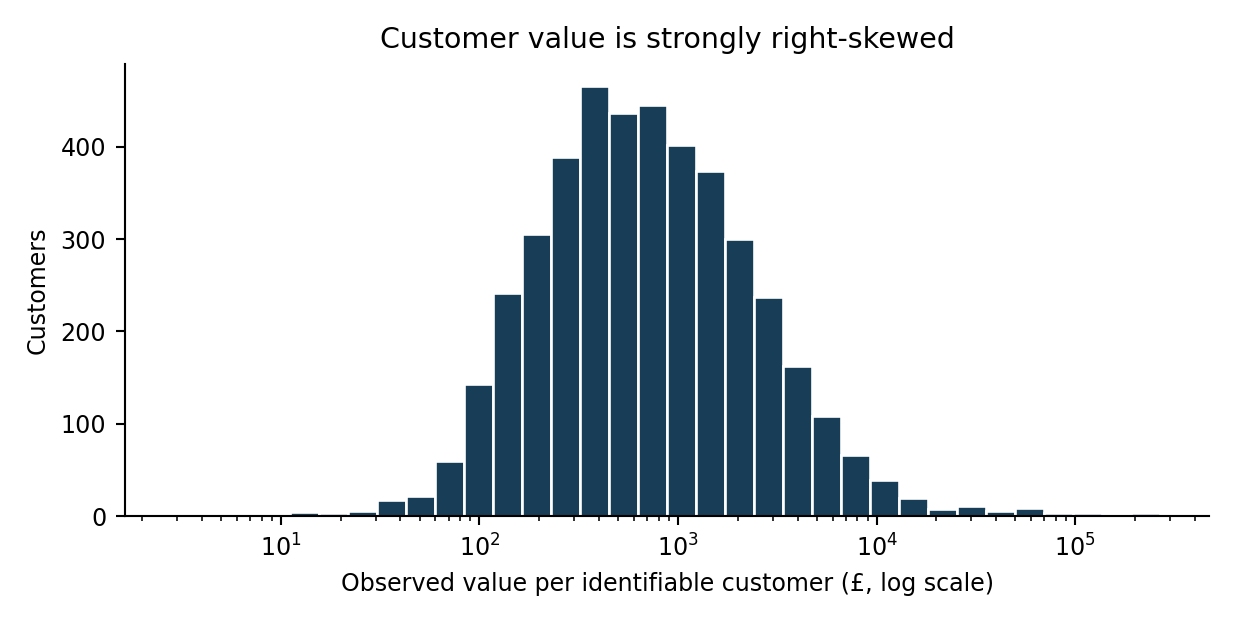
\includegraphics[width=.48\linewidth]{customer_value_distribution.png}\hfill
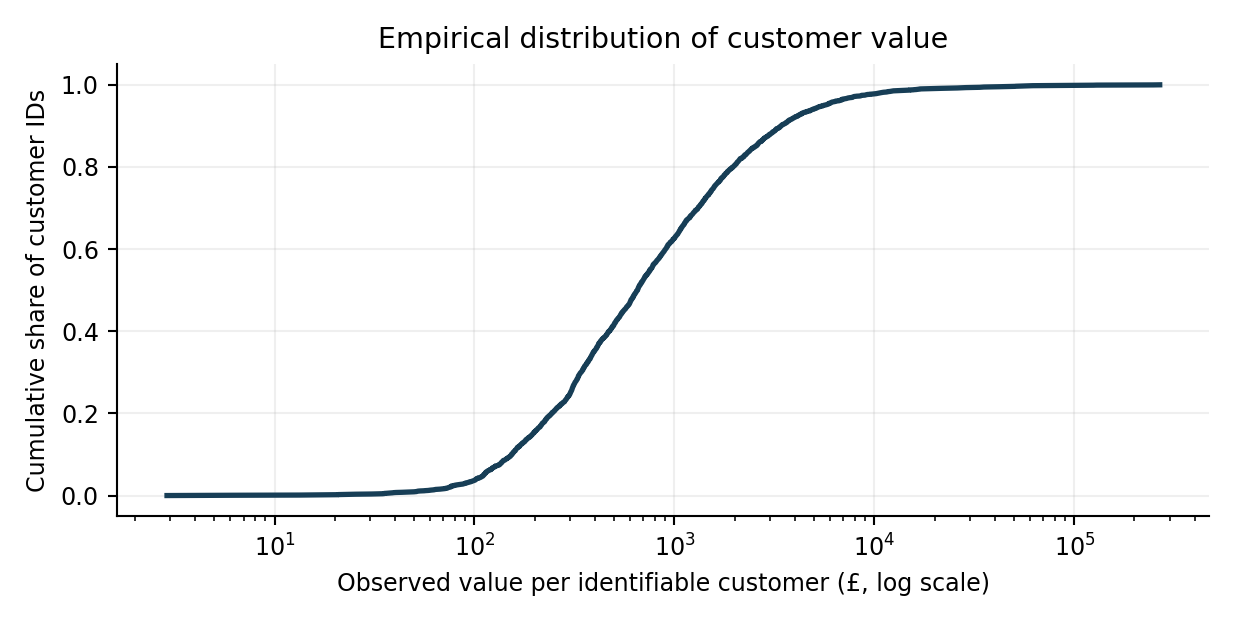
\includegraphics[width=.48\linewidth]{customer_value_ecdf.png}
\caption{Distribution across identifiable customers. The log axis shows the long upper tail without hiding small accounts.}
\end{figure}

\begin{figure}[H]\centering
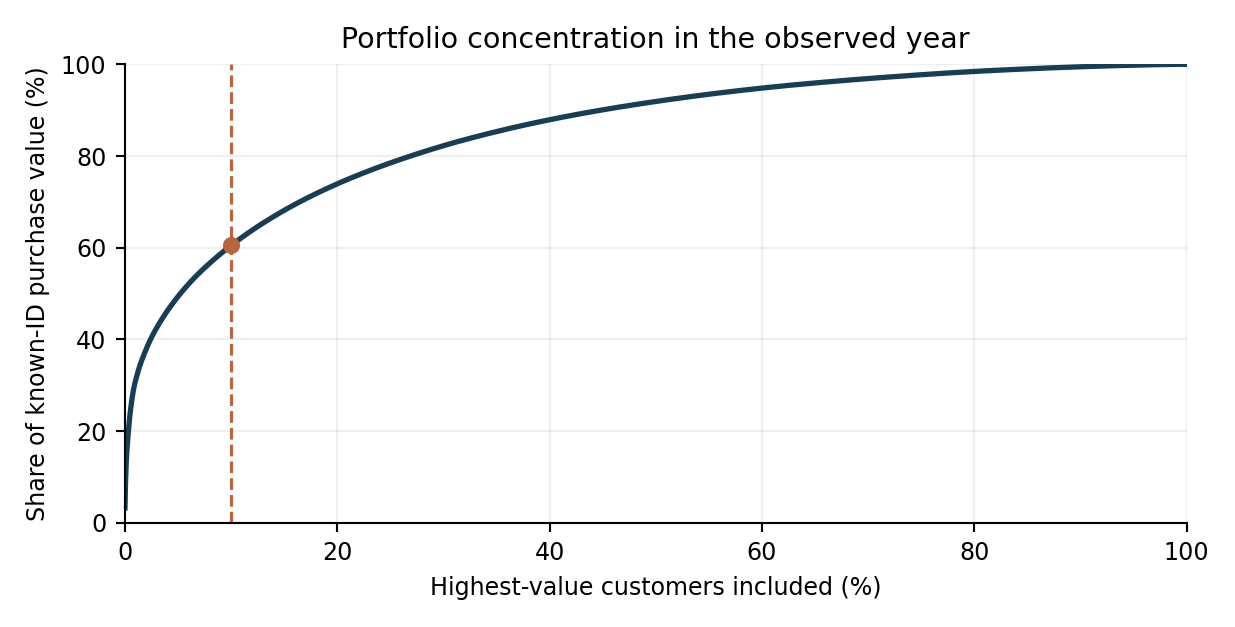
\includegraphics[width=.49\linewidth]{concentration_curve.png}\hfill
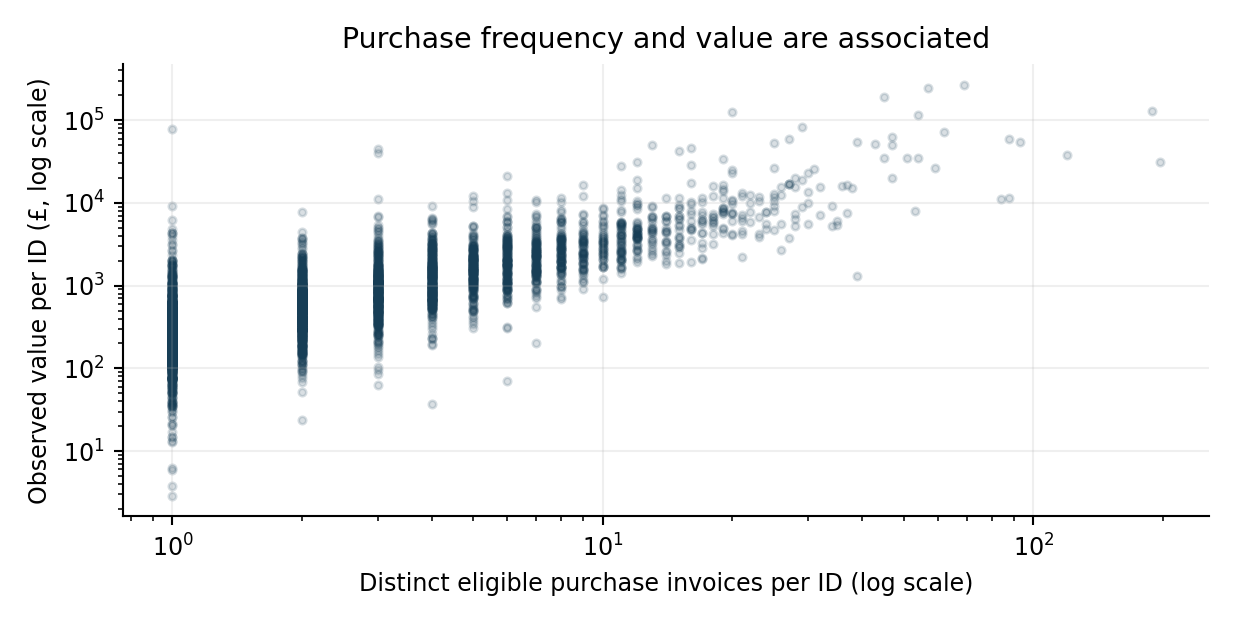
\includegraphics[width=.49\linewidth]{frequency_value_scatter.png}
\caption{Left: cumulative known-ID value by customer rank. Right: distinct eligible invoice count versus observed value, both on log axes.}
\end{figure}

\Needspace{7\baselineskip}Thirty-six per cent of identifiable IDs (1,551) appear in only one \emph{eligible positive purchase invoice} and account for 7.8\% of known-ID value. Multiple lines in one invoice count once; C-coded or unpriced records do not add to this frequency. We compare one invoice with two or more, a split based on observed repeat invoicing rather than an assumed customer type.

\begin{table}[H]\centering\small
\caption{Observed invoice-frequency groups; shares use the same known-ID population.}
\begin{tabular}{@{}lrrrr@{}}\toprule
Group & IDs & Share of IDs & Median value/ID & Share of value \\\midrule
One invoice & 1,551 & 36.1\% & \pounds262.20 & 7.8\% \\
Two or more & 2,742 & 63.9\% & \pounds1,140.28 & 92.2\% \\
\bottomrule\end{tabular}
\end{table}

Invoice count and customer value have Pearson correlation 0.57 and Spearman rank correlation 0.80. The stronger rank association is consistent with a skewed, not simply linear, relationship; it is expected in part because value accumulates across invoices. Neither coefficient establishes why a customer buys more or predicts the effect of a retention action. The one-year observation window also prevents us from calling one-invoice IDs new, lost or permanently inactive customers.

\sectionhead{6\quad Segment checks and missing-ID exposure}
Monthly active customer sets are different, so we \emph{rerank within each month}. These monthly top-decile shares (42.5--57.2\%) are diagnostic comparisons, not the same population as the annual 60.5\% KPI. A month with many short-lived or unidentified accounts may look less concentrated for reasons unrelated to a change in existing customers. We present the known-ID value coverage next to each monthly share rather than interpreting the bars alone.

\begin{table}[H]\centering\small
\caption{Monthly context: distinct identifiable customers and their share of eligible value.}
\begin{tabular}{@{}lrrr@{}}\toprule
Month & Known IDs & ID coverage & Monthly top-decile share \\\midrule
Dec 2010 & 883 & 73.5\% & 49.4\% \\
Jan 2011 & 739 & 84.0\% & 57.2\% \\
Feb 2011 & 757 & 87.5\% & 46.3\% \\
Mar 2011 & 973 & 84.8\% & 47.0\% \\
Apr 2011 & 853 & 88.5\% & 42.5\% \\
May 2011 & 1,054 & 89.4\% & 46.4\% \\
Jun 2011 & 990 & 88.8\% & 54.2\% \\
Jul 2011 & 946 & 86.1\% & 48.4\% \\
Aug 2011 & 933 & 88.0\% & 51.3\% \\
Sep 2011 & 1,259 & 91.5\% & 50.7\% \\
Oct 2011 & 1,361 & 91.1\% & 50.8\% \\
Nov 2011 & 1,660 & 78.6\% & 47.8\% \\
\bottomrule\end{tabular}
\end{table}

\begin{figure}[H]\centering
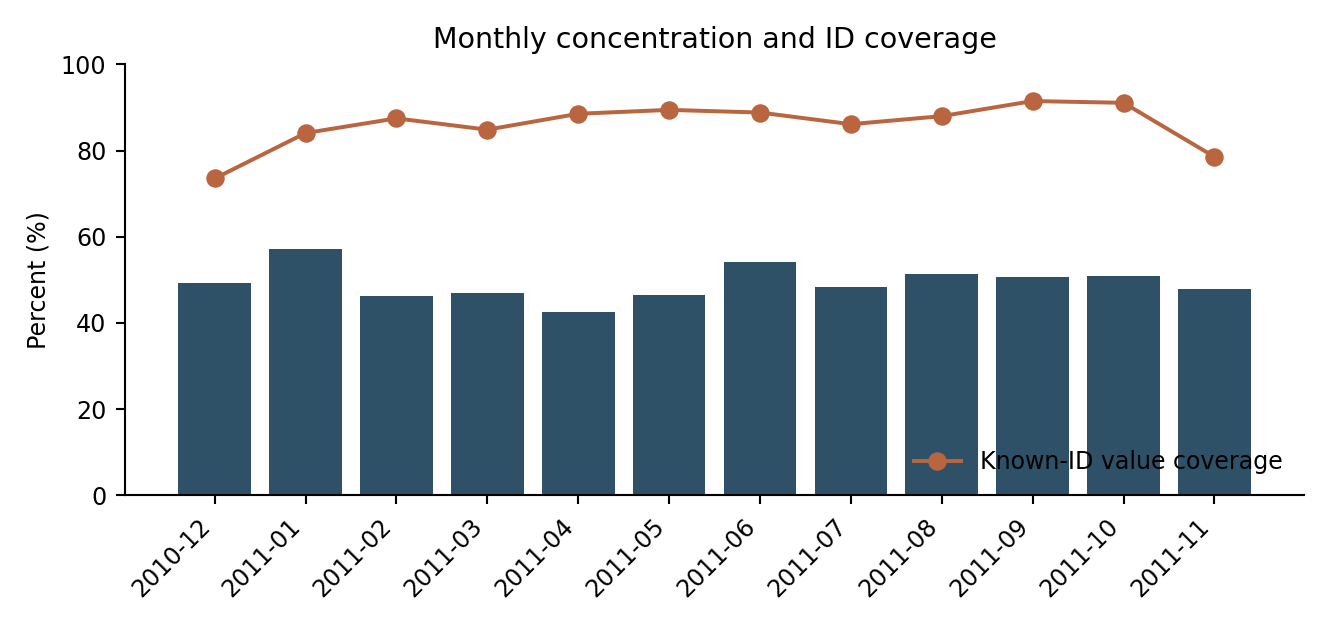
\includegraphics[width=.73\linewidth]{monthly_concentration_coverage.png}
\caption{Monthly concentration (bars) and known-ID value coverage (line). Both depend on the eligible population for that month.}
\end{figure}

Coverage ranges from 73.5\% to 91.5\%; it falls from 91.1\% in October to 78.6\% in November. This is a direct reason not to explain November's lower monthly concentration as a genuine improvement in diversification. Missing IDs could be concentrated in particular invoice types or periods. Because all 1,328 eligible purchase invoices without an ID lack one on every eligible line, within-invoice imputation is unavailable. We cannot show that the known-ID subset represents the missing-ID subset.

As a broad composition check, the United Kingdom has 3,882 identifiable IDs, 83.4\% known-ID value coverage and a 58.4\% within-segment top-decile share. Other recorded customer countries together have 411 IDs, 98.1\% coverage and a 69.2\% share. These are different mixtures of customers and invoice values; country is recorded customer residence, not a verified shipping destination. We do not infer a country effect or compare small countries as though they were equally precise. The complete country table is in \texttt{data/country\_coverage.csv}.

\sectionhead{7\quad Sensitivity, decision and remaining uncertainty}
To test whether the choice of analytical population drives the result, we recalculate the same rank-based indicator under four explicitly labelled alternatives. The broad rule admits charges and other codes, so its similarity to the baseline does not prove that every added line is merchandise. Removing the largest ID changes the population and is only a dependence diagnostic.

\begin{table}[H]\centering\small
\caption{Sensitivity of the annual concentration measure. Alternatives are not silent corrections.}
\begin{tabularx}{\linewidth}{@{}Xrrr@{}}\toprule
Population & IDs & Top-decile share & ID coverage \\\midrule
Baseline merchandise rule & 4,293 & 60.50\% & 85.66\% \\
Drop exact repeat rows & 4,293 & 60.58\% & 85.63\% \\
Strict five-digit codes & 4,273 & 60.41\% & 85.68\% \\
All positive priced stock codes & 4,297 & 60.58\% & 83.70\% \\
Remove largest known ID & 4,292 & 59.22\% & 85.25\% \\
\bottomrule\end{tabularx}
\end{table}

Exact-row removal changes the indicator by only 0.08 percentage points, while dropping the largest ID changes it by 1.28 points. These checks support the narrower statement that the \emph{measured known-ID concentration} is fairly stable under these four specific alternatives. They do not resolve whether exact repeats are true events, whether the code rule excludes valid products or how the 14.3\% of eligible value without IDs would affect the portfolio. A small aggregate change could still alter individual account ranks, so a future operational use should compare account-level classifications as well.

\subhead{Main EDA insight and decision}
The portfolio is concentrated across a \emph{group}, not solely one extreme record: the highest-value 1\% of known IDs (43) provide 30.9\% of known-ID value, while the single largest ID provides 3.25\%. Customers observed in at least two eligible invoices provide 92.2\% of known-ID value, whereas the 36.1\% observed in one invoice provide only 7.8\%. Together with the long-tailed customer-value distribution, this suggests that a small set of repeatedly observed accounts explains much of the recorded value. It does \emph{not} establish loyalty, future purchasing or the effect of a retention campaign.

We would use this insight to prioritise a qualitative review of major accounts \emph{and} the ID-capture process. We would not call 60.5\% ``too high'' without a benchmark or business risk tolerance, nor infer profitability or revenue at risk. A future refresh would require stable identifiers, a comparable window, documented product codes and, for financial decisions, reconciled payments, costs and cancellation links. A dashboard should display concentration, ID coverage and population counts together; hiding coverage would make the KPI easier to misread.

\sectionhead{8\quad Continuation beyond C1}
Our selected line remains viable because it has an explicit invoice-line input, reproducible customer aggregation and measured ID coverage. A change to Candidate B would require a trustworthy link from each C record to its original purchase before estimating matched cancellations. The next stage should first confirm product-code definitions and identity capture, not assume that the present KPI is a finished management system.

\subhead{A concrete possible ML task}
We propose exploratory \emph{customer-profile clustering} for a future account-review exercise. One case would be one known \texttt{CustomerID} at a fixed monthly cut-off; inputs available from this source before that cut-off are days since last eligible purchase, distinct eligible invoices in a trailing window, observed positive value and mean invoice value. We would compare whether interpretable profiles separate low-frequency from repeatedly observed high-value accounts and whether assignments remain stable over successive cut-offs. Clustering has no observed outcome label; its decision value would be a more structured qualitative review, not a forecast of profit or a rule to contact customers automatically. The 14.3\% of eligible value without IDs cannot enter these profiles. Longer, recent history and verified stable customer identifiers are required for prospective use; payments, costs and linked cancellations would be needed before a financial-value interpretation. Features computed after a proposed decision date must not be used as if they were available then. Transaction-based customer segmentation is supported as a research direction, not as validation of our future clusters.\source{3} C1 trains no model and makes no performance claim.

\subhead{Proposed dashboard use}
The proposed user is a commercial analyst reviewing the account portfolio each month. The first view would show trailing-12-month $K_{10}$, $C_{ID}$, $N$ and the known-ID value denominator together; hiding coverage would make concentration easy to misread. Monthly diagnostics would show complete-month periods, monthly re-ranked concentration, ID coverage and customer counts side by side. An invoice-frequency comparison and a drill-down to major IDs and their eligible invoices would support checking whether the aggregate change comes from a few accounts or recording rules. A separate exception view would show blank IDs, C-coded and other retained lines without adding them to positive purchase value. These displays follow the EDA's long upper tail, repeat-invoice association and November coverage drop; they would support investigation, not an automatic intervention. No dashboard is built in C1.

\sectionhead{9\quad Process record}
\subhead{Decisions and checks}
The uncleaned 12-month CSV and source manifest are in \texttt{data/}. Running \texttt{analysis/c1\_analysis.py} produces the one-to-one flag file, customer and invoice aggregates, monthly and country summaries, sensitivity tables, figures and \texttt{report\_metrics.json}. The executed \texttt{analysis/C1\_customer\_portfolio.ipynb} saves the checks and results. The table records the consequential choices rather than every command.

\begin{table}[H]\centering\small
\caption{Decision trail with alternatives, checks and submitted evidence.}
\begin{tabularx}{\linewidth}{@{}>{\raggedright\arraybackslash}p{1.7cm}>{\raggedright\arraybackslash}p{3.0cm}X@{}}\toprule
Stage & Choice versus alternative & Reason, check, outcome and evidence location \\\midrule
W1 & Advance A over B & Known IDs and priced invoices support a ranked portfolio measure; B lacks purchase links. Section 1 records the comparison; \path{data/report_metrics.json} checks the denominator. \\
C1 scope & Use twelve full months & The final December has only nine days. We retained 516,384 rows through November 2011; \path{analysis/c1_analysis.py} asserts bounds and count. One cycle cannot establish seasonality. \\
C1 preparation & Keep repeats; do not fill IDs or prices & No line ID resolves repeats, and 1,328 eligible invoices have entirely blank IDs. There is no observed replacement price. Flags remain in \path{data/prepared_lines.csv}; repeat removal changes $K_{10}$ by 0.08 points. \\
C1 EDA & Retain large IDs; display coverage & Removing the largest ID lowers $K_{10}$ to 59.22\%; monthly coverage falls from 91.1\% to 78.6\% in October--November. See Sections 5--7 and \path{data/sensitivity.csv}. \\
\bottomrule\end{tabularx}
\end{table}

\Needspace{8\baselineskip}\subhead{Instructor feedback and response}
No case-specific instructor feedback on the W1 A/B selection or this C1 analysis was available to us by 27 September 2026. We therefore retain A provisionally, with the measurable denominator and missing-ID guardrail above. We will ask whether this retail case fits the C1 domain expectation and whether positive recorded purchase value is an acceptable interim measure. Until then, we make no MINSAL connection, net-revenue claim or automatic intervention rule. The question and provisional response are recorded here rather than presented as advice already received.

\subhead{Individual contributions}
\begin{table}[H]\centering\small
\caption{Team account of contributions to the analytical choices.}
\begin{tabularx}{\linewidth}{@{}p{2.4cm}X@{}}\toprule
Member & Contribution and evidence in this submission \\\midrule
Mois\'{e}s Medina & Jointly framed the proposed decision and compared alternatives; investigated Candidate A, the customer-ranking denominator, ID coverage and sensitivity. Evidence: Sections 1--2 and 5--7; \texttt{data/report\_metrics.json} and \texttt{data/sensitivity.csv}. \\
Ignacia Castillo & Jointly framed the proposed decision; investigated Candidate B, the limits of C-coded records and the business interpretation of the alternative. Evidence: Section 1 comparison, Sections 3--4 treatment of C records, and the limitations in Section 7. \\
\bottomrule\end{tabularx}
\end{table}

\subhead{AI use and verification}
As in W1, we used OpenAI Codex to prepare first drafts of the written report and Python code, including LaTeX formatting and possible EDA displays. These drafts were working material, not our evidence or final business analysis. One request was, in translation, ``build and validate the analytical dataset, do directed EDA, and define the KPI and its rule of use.'' The generated code proposed explicit \texttt{eligible\_purchase} and \texttt{row\_group} flags and a top-decile calculation. We accepted these structures after checking the 516,384-row partition, positive eligible values, invoice-to-ID consistency and equality of the report numbers with generated CSV/JSON outputs. Another request asked that every exclusion and retention choice have a business reason. We revised the draft to keep ambiguous repeats, missing-ID value and large accounts visible, with sensitivity tests rather than silent deletion. We rejected interpretations that zero prices were proven discounts, that C-coded records could be netted to original purchases, or that repeat invoices proved loyalty. We chose the business question, analytical population, KPI scope and decision implications, and we made the final interpretation of the results. The notebook was executed from first cell to last with saved outputs.\source{5}

\subhead{Individual reflection}
\textbf{Mois\'{e}s.} My main contribution was narrowing Candidate A to a ranking with an explicit known-ID denominator. I learned that a percentage is only useful when its population and coverage are stated together. The unresolved uncertainty is whether the missing-ID purchases differ systematically from identified accounts.

\textbf{Ignacia.} My main contribution was testing what the C prefix permits us to say about Candidate B and challenging a matched-cancellation interpretation. I learned to distinguish a source flag from a verified business event and to keep alternative explanations open. The unresolved uncertainty is how non-C negative quantities and special stock codes should be classified with an operational codebook.

\sectionhead{References}
\begingroup\small
\begin{enumerate}[leftmargin=1.4em,itemsep=0em,parsep=0em]
\item Chen, D. (2015). \emph{Online Retail} [dataset]. UCI Machine Learning Repository. DOI: \href{https://doi.org/10.24432/C5BW33}{10.24432/C5BW33}. Dataset, dictionary and CC BY 4.0 licence: \url{https://archive.ics.uci.edu/dataset/352/online-retail}. Accessed 27 September 2026.
\item Fontecilla, T. (2026). \emph{Business Intelligence: From strategy to measurable evidence; Data preparation; EDA after data validation}. Course lecture materials, Universidad del Desarrollo. Used for the strategy-to-KPI chain, validation order and robust EDA.
\item Chen, D., Sain, S. L., and Guo, K. (2012). ``Data mining for the online retail industry: A case study of RFM model-based customer segmentation using data mining.'' \emph{Journal of Database Marketing \& Customer Strategy Management}, 19, 197--208. DOI: \href{https://doi.org/10.1057/dbm.2012.17}{10.1057/dbm.2012.17}. Published online 27 August 2012.
\item Han, Z., Yu, C., Li, Y., Shi, J., et al. (2023). ``Customer concentration and supplier financial performance: An inverted U-shaped relationship.'' \emph{Industrial Marketing Management}, 113, 138--152. DOI: \href{https://doi.org/10.1016/j.indmarman.2023.06.003}{10.1016/j.indmarman.2023.06.003}. Used only to motivate the bounded concentration question; the study population differs from this case.
\item Fontecilla, T. (2026). \emph{C1: From the W1 project to defensible evidence. Brief and rubric}, IIB423T-1, Universidad del Desarrollo. Version supplied for the 29 September 2026 assessment; consulted 27 September 2026.
\end{enumerate}
\endgroup
\end{document}
